\chapter{taxize: taxonomic search and retrieval in R}
\label{sec:taxize} 
 
\bigskip
Scott A. Chamberlain\textsuperscript{a} \& Eduard Szöcs\textsuperscript{b}

\bigskip
\small
\noindent 
\textsuperscript{a}Biology Department, Simon Fraser University, Burnaby, BC, Canada,\\
\textsuperscript{b}Institute for Environmental Sciences, University Koblenz-Landau, Landau, Germany \\

\bigskip 
\normalsize
\noindent 
Adapted from the article published in 2013 in \emph{F1000Research}, 2.191.

\bigskip
\noindent
This chapter reflects the software state in 2013.
In the meantime there have been many changes to taxize, so that not all parts presented here work anymore. 
For a more recent description please visit the project homepage \url{https://github.com/ropensci/taxize}.


\newpage


%% ----------------------------------------------------------------------------
% be sloppy in this chapter
\begin{sloppypar}
\section{Abstract} 
\label{sec:taxize:abstract} 
All species are hierarchically related to one another, and we use taxonomic names to label the nodes in this hierarchy. 
Taxonomic data is becoming increasingly available on the web, but scientists need a way to access it in a programmatic fashion that's simple and reproducible. 
We have developed taxize, an open-source software package for the R language (freely available from \url{http://cran.r-project.org/web/packages/taxize}). 
taxize provides simple, programmatic access to taxonomic data for 13 data sources around the web. 
We discuss the need for a taxonomic toolbelt in R, and outline a suite of use cases for which taxize is ideally suited (including a full workflow as an appendix). 
The taxize package facilitates open and reproducible science by allowing taxonomic data collection to be done in the open-source R platform.

%% ----------------------------------------------------------------------------
\section{Introduction} 
\label{sec:taxize:introduction} 
Evolution by natural selection has led to a hierarchical relationship among all living organisms.  
Thus, species are categorized using a taxonomic hierarchy, starting with the binomial species name (e.g, \emph{Homo sapiens}), moving up to genus (\emph{Homo}), then family (\emph{Hominidae}), and on up to Domain (\emph{Eukarya}). 
Although taxonomic classifications are human constructs created to understand the real phylogeny of life \citep{benton2000}, they are nonetheless essential to organize the vast diversity of organisms. 
Biologists, whether studying organisms at the cell, organismal, or community level, can put their study objects into taxonomic context, allowing them to infer close and distant relatives, find relevant literature, and more. 

The use of taxonomic names is, unfortunately, not straightforward. 
Taxonomic names often vary due to name revisions at the generic or specific levels, lumping or splitting lower taxa (genera, species) among higher taxa (families), and name spelling changes. 
For example, a study found that a compilation of 308,000 plant observations from 51 digitized herbarium records had 22,100 unique taxon names, of which only ~13,000 were accepted names \citep{weiser2007,boyle2013}. 
In addition, there is no one authoritative source of taxonomic names for all taxa - although, there are taxon specific sources that are used by many scientists. 
Different sources (e.g., uBio [Universal Biological Indexer and Organizer], Tropicos, ITIS [Integrated Taxonomic Information Service]) may use different accepted names for the same taxon. 
For example, while ITIS has \emph{Helianthus x glaucus} as an accepted name, The Plant List (\url{http://www.theplantlist.org}) gives that name as unresolved. But \emph{Helianthus glaucus} is an accepted name in The Plant List, while ITIS does not list this name. 

One attempt to help inconsistencies in taxonomy is the use of numeric codes. 
For example, ITIS assigns a Taxonomic Serial Number (TSN) to each taxon, while uBio assigns each taxon a NameBank identifier (namebankID), and Tropicos assigns their own identifier to each taxon. 
Codes are helpful within a database as they can easily refer to, for example, \emph{Helianthus annuus} with a code like 123456 instead of its whole name. 
However, each database uses their own code; in this case for \emph{Helianthus annuus}, ITIS uses 36616, uBio uses 2658020, and Tropicos uses 40022652. 
As there are no universal codes for taxa across databases, this can lead to additional confusion. 
Last, name comparisons across databases have to be done with the actual names, not the codes. 

Taxonomic data is getting easier to obtain through the web (e.g., \url{http://eol.org/}). 
However, there are a number of good reasons to obtain taxonomic information programatically rather than through a web interface. 
First, if you have more than a few names to look up on a website, it can take quite a long time to enter each name, get data, and repeat for each species. 
Programatically getting taxonomic names solves the problem by looping over a list of names. In addition, doing taxonomic searching, etc. becomes reproducible. 
With increasing reports of irreproducibility in science \citep{stodden2010,zimmer2012}, it is extremely important to make science workflows repeatable.

The R language is widely used by biologists, and now has over 5,000 packages on the Comprehensive R Archive Network (CRAN) to extend R. 
R is great for manipulating, visualizing and fitting statistical models to data. 
Gentleman et al. \citet{gentleman_bioconductor:_2004} give a detailed discussion of advantages of R in computational biology. Getting data from the web will be increasingly common as more and more data gets moved to the cloud. 
Therefore, there is a need to get data from the web directly into R. 
Increasingly, data is available from the web via application programming interfaces (API). 
These allow computers to talk to one another using code that is not human readable, but is machine readable. 
Web APIs often define a number of methods that allow users to search for a species name, or retrieve the synonyms for a species name, for example. 
A further advantage of APIs is that they are language agnostic, meaning that data can be consumed in almost any computing context, allowing users to interact with the web API without having to know the details of the code. 
Moreover data can be accessed from every computer, whereas for example an Excel file can only be opened in a few programs. 

The goal of taxize is to make many use cases that involve retrieving and resolving taxonomic names easy and reproducible. 
In taxize, we have written a suite of R functions that interact with many taxonomic data sources via their web APIs (Table~\ref{tab:taxize:fnx}). 
The interface to each function is usually a simple list of species names, just as a user would enter when interacting with a website. 
Therefore, we hope that moving from a web to an R interface for taxonomic names will be relatively seamless (if one is already nominally familiar with R). 

Here, we justify the need for programmatic taxonomic resolution tools like taxize, discuss our data sources, and run through a suite of use cases to demonstrate the variety of ways that users can use taxize.

{\small
\begin{longtable}{p{3.5cm}p{5cm}p{5cm}}
\caption{Some key functions in taxize, what they do, and their data sources}\\
\hline
Function name & What it does & Source \\
\hline
\endfirsthead
{\tablename\ \thetable\ -- \textit{Cont.}} \\
\hline
Function name & What it does & Source \\
\hline
\endhead
apg\_lookup() & Changes names to match the APGIII list & Angiosperm Phylogeny Group \url{http://www.mobot.org/MOBOT/research/APweb/}  \\
classification() & Upstream classification & Various  \\
col\_children() & Direct children & Catalogue of Life \newline \url{http://www.catalogueoflife.org/}  \\
col\_downstream() & Downstream taxa to specified rank & Catalogue of Life \newline \url{http://www.catalogueoflife.org/}  \\
eol\_hierarchy() & Upstream classification & Encyclopedia of Life \newline \url{http://eol.org/}  \\
eol\_search() & Search EOL taxon information & Encyclopedia of Life \newline \url{http://eol.org/}  \\
get\_seqs() & Get NCBI sequences & National Center for Biotechnology Information \citep{federhen2012}  \\
get\_tsn() & Get ITIS TSN & Integrated Taxonomic Information System \newline \url{http://www.itis.gov/}  \\
get\_uid() & Get NCBI UID & National Center for Biotechnology Information \citep{federhen2012}  \\
gisd\_isinvasive() & Invasiveness status & Global Invasive Species Database \newline \url{http://www.issg.org/database/welcome/}  \\
gni\_parse() & Parse scientific names into components & Global Names Index \newline \url{http://gni.globalnames.org/}   \\
gni\_search() & Search EOL's global names index & Global Names Index \newline \url{http://gni.globalnames.org/}   \\
gnr\_resolve() & Resolve names using EOL's global names index & Global Names Resolver \newline \url{http://resolver.globalnames.org/}  \\
itis\_downstream() & Downstream taxa to specified rank & Integrated Taxonomic Information System \newline \url{http://www.itis.gov/}  \\
iucn\_status() & IUCN status & IUCN Red List \newline \url{http://www.iucnredlist.org}  \\
phylomatic\_tree() & Get a plant Phylogeny & Phylomatic \citep{webb2005}  \\
plantminer() & Search Plantminer & Plantminer \citep{carvalho2010plantminer}   \\
searchby\-commonname() & Search ITIS by common name & Integrated Taxonomic Information System \newline \url{http://www.itis.gov/}  \\
searchby\-scientificname() & Search ITIS by scientific name & Integrated Taxonomic Information System \newline \url{http://www.itis.gov/}  \\
tax\_name() & Get taxonomic name for specific rank & Various  \\
tax\_rank() & Get rank of a taxonomic name & Various  \\
tnrs() & Resolve names using iPlant & iPlant Taxonomic Name Resolution Service \newline \url{http://tnrs.iplantcollaborative.org/}  \\
tp\_accepted\-names() & Check for accepted names using Tropicos & Tropicos \newline \url{http://www.tropicos.org/}  \\
tpl\_search() & Search the Plant List & The Plant List \newline \url{http://www.theplantlist.org}  \\
ubio\_namebank() & Search uBio & uBio \newline \url{http://www.ubio.org/index.php?pagename=sample_tools}  \\
\hline
\label{tab:taxize:fnx}
\end{longtable}
}

%% ----------------------------------------------------------------------------
\section{Why do we need taxize?}
\label{sec:taxize:why} 
There is a large suite of applications developed around the problem of searching for, resolving, and getting higher taxonomy for species names. 
For example, Linnaeus (\url{http://linnaeus.sourceforge.net/}) provides the ability to search for taxonomic names in documents and normalize those names found. 
In addition, there are many web interfaces to search for and normalize names such as Encyclopedia of Life's Global Names Resolver (\url{http://resolver.globalnames.org/}), uBio tools (\url{www.ubio.org/index.php?pagename=sample_tools}), and iPlant's Taxonomic Name Resolution Service (\url{http://tnrs.iplantcollaborative.org/}). 

All of these data repositories provide ways to search for taxonomic names and resolve them in some cases. 
However, scientists ideally need a tool that is free and can be used programmatically, thereby facilitating reproducible research. 
The goal of taxize is to facilitate the creation of reproducible and easy to use workflows for searching for taxonomic names, resolving them, getting higher taxonomic names, and other tasks related to research dealing with species.

%% ----------------------------------------------------------------------------
\section{Data sources and package details}
\label{sec:taxize:sources} 
taxize uses many data sources (Table~\ref{tab:taxize:fnx}), and more can be easily added. 
There are two common tasks provided by the data sources: name search and name resolution. 
Other functionality in taxize includes retrieving a classification tree for a species, or retrieving child taxa of a focal taxon. O
ne of the data sources (Phylomatic) returns phylogenies, while another (NCBI) returns genetic sequence data. 
However, there are other R packages that are focused solely on sequence data, such as rsnps \citep{chamberlain2013}, rentrez \citep{winter2013}, BoSSA \citep{lefeuvre2010}, and ape \citep{paradis2004}, so taxize does not venture deeply into these other domains. 

Some of the data sources taxize interacts with require authentication. 
That is, in addition to the search terms the user provides (e.g., \emph{Homo sapiens}), the data provider requires an alphanumeric identification key. 
This is necessary in some cases so that API providers can 1) better prevent databases crashing from too many requests, 2) collect analytics on requests to their API to provide better performance, etc., and 3) provide user level modification of rules for interacting with the API. 
The services that require an API key in taxize are: Encyclopedia of Life (EOL) (\url{http://eol.org/}), the Universal Biological Indexer and Organizer (uBio) (\url{http://www.ubio.org/index.php?pagename=sample_tools}), Tropicos (\url{http://www.tropicos.org/}), and Plantminer \citep{carvalho2010plantminer}. 
One can easily obtain API keys by visiting the website of each service (see Table~\ref{tab:taxize:fnx} for links to each site). 
There are two typical ways of using API keys. 
First, you can pass in your API key in a function call (e.g., \emph{ubio\_namebank(srchName='Ursus americanus', key='your\_alphanumeric\_key')}). 
Second, you can store your key in the .Rprofile file, which is a common place to store settings. We recommend the second option as it simplifies function calls as taxize detects the stored keys.

taxize would not have been possible without the work of others. 
taxize uses httr \citep{httr} and RCurl \citep{rcurl} for performing calls to web APIs, XML \citep{xml} for parsing XML, RJSONIO \citep{rjsonio} for parsing JSON, and stringr \citep{stringr} and plyr \citep{plyr} for manipulating data.
  
New data sources can be added: for example, we plan to add the following sources: Wikispecies (\url{https://species.wikimedia.org}) and The Tree of Life (\url{http://tolweb.org/tree/}). 
A connection to \url{www.freshwaterecology.info} (a database with autecological characteristics, ecological preferences and biological traits as well as distribution patterns of more than 12,000 European freshwater organisms belonging to fish, macro-invertebrates, macrophytes, diatoms and phytoplankton) will be finished when their new API is released. 
In addition, the authors welcome further suggestions of data sources to be added.


%% ----------------------------------------------------------------------------
\section{Use cases}
\subsection{First, install taxize}

First, one must install and load taxize into the R session.

\begin{knitrout}
\small
\definecolor{shadecolor}{rgb}{0.969, 0.969, 0.969}
\color{fgcolor}
\begin{kframe}
\begin{alltt}
\hlkwd{install.packages}\hlstd{(}\hlstr{"taxize"}\hlstd{)}
\hlkwd{library}\hlstd{(taxize)}
\end{alltt}
\end{kframe}
\end{knitrout}

Advanced users can also download and install the latest development copy from GitHub \url{https://github.com/ropensci/taxize}, also permanently available at \url{http://dx.doi.org/10.5281/zenodo.7097}.


\subsection{Resolve taxonomic names}
This is a common task in biology. 
We often have a list of species names and we want to know a) if we have the most up to date names, b) if our names are spelled correctly, and c) the scientific name for a common name. 
One way to resolve names is via the Global Names Resolver (GNR) service provided by the Encyclopedia of Life (\url{http://resolver.globalnames.org/}). 
Here, on can search for two misspelled names:

\begin{knitrout}
\small
\definecolor{shadecolor}{rgb}{0.969, 0.969, 0.969}
\color{fgcolor}
\begin{kframe}
\begin{alltt}
\hlstd{temp} \hlkwb{<-} \hlkwd{gnr_resolve}\hlstd{(}\hlkwc{names} \hlstd{=} \hlkwd{c}\hlstd{(}\hlstr{"Helianthos annus"}\hlstd{,}
                              \hlstr{"Homo saapiens"}\hlstd{))}
\hlstd{temp[ ,} \hlopt{-}\hlkwd{c}\hlstd{(}\hlnum{1}\hlstd{,}\hlnum{4}\hlstd{)]}
\end{alltt}
\begin{verbatim}
#                  matched_name       data_source_title
# 1        Helianthus annuus L.       Catalogue of Life
# 2            Helianthus annus GBIF Taxonomic Backbone
# 3            Helianthus annus                     EOL
# 4         Helianthus annus L.                     EOL
# 5            Helianthus annus           uBio NameBank
# 6 Homo sapiens Linnaeus, 1758       Catalogue of Life
\end{verbatim}
\end{kframe}
\end{knitrout}

The correct spellings are \emph{Helianthus annuus} and \emph{Homo sapiens}. 
Another approach uses the Taxonomic Name Resolution Service via the Taxosaurus API (\url{http://taxosaurus.org/}) developed by iPLant and the Phylotastic organization. 
In this example is a list of species names, some of which are misspelled, and then call the API with the \emph{tnrs} function.

\begin{knitrout}
\small
\definecolor{shadecolor}{rgb}{0.969, 0.969, 0.969}
\color{fgcolor}
\begin{kframe}
\begin{alltt}
\hlstd{mynames} \hlkwb{<-} \hlkwd{c}\hlstd{(}\hlstr{"Helianthus annuus"}\hlstd{,} \hlstr{"Pinus contort"}\hlstd{,}
             \hlstr{"Poa anua"}\hlstd{,} \hlstr{"Abis magnifica"}\hlstd{,} \hlstr{"Rosa california"}\hlstd{,}
             \hlstr{"Festuca arundinace"}\hlstd{,} \hlstr{"Sorbus occidentalos"}\hlstd{,}
             \hlstr{"Madia sateva"}\hlstd{)}
\hlkwd{tnrs}\hlstd{(}\hlkwc{query} \hlstd{= mynames)[ ,} \hlopt{-}\hlkwd{c}\hlstd{(}\hlnum{5}\hlopt{:}\hlnum{7}\hlstd{)]}
\end{alltt}
\begin{verbatim}
#          submittedName        acceptedName    sourceId score
# 9    Helianthus annuus   Helianthus annuus iPlant_TNRS     1
# 10   Helianthus annuus   Helianthus annuus        NCBI     1
# 4        Pinus contort      Pinus contorta iPlant_TNRS  0.98
# 5             Poa anua           Poa annua iPlant_TNRS  0.96
# 3       Abis magnifica     Abies magnifica iPlant_TNRS  0.96
# 7      Rosa california    Rosa californica iPlant_TNRS  0.99
# 8      Rosa california          California        NCBI     1
# 2   Festuca arundinace Festuca arundinacea iPlant_TNRS  0.99
# 1  Sorbus occidentalos Sorbus occidentalis iPlant_TNRS  0.99
# 6         Madia sateva        Madia sativa iPlant_TNRS  0.97
\end{verbatim}
\end{kframe}
\end{knitrout}


It turns out there are a few corrections: e.g., \emph{Madia sateva} should be \emph{Madia sativa}, and \emph{Rosa california} should be \emph{Rosa californica}. 
Note that this search worked because fuzzy matching was employed to retrieve names that were close, but not exact matches. 
Fuzzy matching is only available for plants in the TNRS service, so we advise using EOL's Global Names Resolver if you need to resolve animal names.

taxize takes the approach that the user should be able to make decisions about what resource to trust, rather than making the decision on behalf of the user. 
Both the EOL GNR and the TNRS services provide data from a variety of data sources. 
The user may trust a specific data source, and thus may want to use the names from that data source. 
In the future, we may provide the ability for taxize to suggest the best match from a variety of sources.

Another common use case is when there are many synonyms for a species. 
In this example, there are six synonyms of the currently accepted name for a species. 

\begin{knitrout}
\small
\definecolor{shadecolor}{rgb}{0.969, 0.969, 0.969}
\color{fgcolor}
\begin{kframe}
\begin{alltt}
\hlkwd{library}\hlstd{(plyr)}
\hlstd{mynames} \hlkwb{<-} \hlkwd{c}\hlstd{(}\hlstr{"Helianthus annuus ssp. jaegeri"}\hlstd{,}
             \hlstr{"Helianthus annuus ssp. lenticularis"}\hlstd{,}
             \hlstr{"Helianthus annuus ssp. texanus"}\hlstd{,}
             \hlstr{"Helianthus annuus var. lenticularis"}\hlstd{,}
             \hlstr{"Helianthus annuus var. macrocarpus"}\hlstd{,}
             \hlstr{"Helianthus annuus var. texanus"}\hlstd{)}
\hlstd{tsn} \hlkwb{<-} \hlkwd{get_tsn}\hlstd{(mynames)}
\hlkwd{ldply}\hlstd{(tsn, itis_acceptname)}
\end{alltt}
\begin{verbatim}
#   submittedTsn      acceptedName acceptedTsn
# 1       525928 Helianthus annuus       36616
# 2       525929 Helianthus annuus       36616
# 3       525930 Helianthus annuus       36616
# 4       536095 Helianthus annuus       36616
# 5       536096 Helianthus annuus       36616
# 6       536097 Helianthus annuus       36616
\end{verbatim}
\end{kframe}
\end{knitrout}


\subsection{Retrieve higher taxonomic names}
Another task biologists often face is getting higher taxonomic names for a taxa list. 
Having the higher taxonomy allows you to put into context the relationships of your species list. 
For example, you may find out that species A and species B are in Family C, which may lead to some interesting insight, as opposed to not knowing that Species A and B are closely related.
 This also makes it easy to aggregate/standardize data to a specific taxonomic level (e.g., family level) or to match data to other databases with different taxonomic resolution (e.g., trait databases).

A number of data sources in taxize provide the capability to retrieve higher taxonomic names, but we will highlight two of the more useful ones: Integrated Taxonomic Information System (ITIS) (\url{http://www.itis.gov/}) and National Center for Biotechnology Information (NCBI) \citep{federhen2012}.
First, search for two species, \emph{Abies procera} and \emph{Pinus contorta} within ITIS.

\begin{knitrout}
\small
\definecolor{shadecolor}{rgb}{0.969, 0.969, 0.969}
\color{fgcolor}
\begin{kframe}
\begin{alltt}
\hlstd{specieslist} \hlkwb{<-} \hlkwd{c}\hlstd{(}\hlstr{"Abies procera"}\hlstd{,} \hlstr{"Pinus contorta"}\hlstd{)}
\hlkwd{classification}\hlstd{(specieslist,} \hlkwc{db} \hlstd{=} \hlstr{"itis"}\hlstd{)}
\end{alltt}
\begin{verbatim}
# $`Abies procera`
#         rankName       taxonName    tsn
# 1        Kingdom         Plantae 202422
# 2     Subkingdom  Viridaeplantae 846492
# 3   Infrakingdom    Streptophyta 846494
# 4       Division    Tracheophyta 846496
# 5    Subdivision Spermatophytina 846504
# 6  Infradivision    Gymnospermae 846506
# 7          Class       Pinopsida 500009
# 8          Order         Pinales 500028
# 9         Family        Pinaceae  18030
# 10         Genus           Abies  18031
# 11       Species   Abies procera 181835
# 
# $`Pinus contorta`
#         rankName       taxonName    tsn
# 1        Kingdom         Plantae 202422
# 2     Subkingdom  Viridaeplantae 846492
# 3   Infrakingdom    Streptophyta 846494
# 4       Division    Tracheophyta 846496
# 5    Subdivision Spermatophytina 846504
# 6  Infradivision    Gymnospermae 846506
# 7          Class       Pinopsida 500009
# 8          Order         Pinales 500028
# 9         Family        Pinaceae  18030
# 10         Genus           Pinus  18035
# 11       Species  Pinus contorta 183327
\end{verbatim}
\end{kframe}
\end{knitrout}

It turns out both species are in the family Pinaceae.
You can also get this type of information from the NCBI by excuting the following code in R: \emph{classification(specieslist, db = 'ncbi')}.

Instead of a full classification, you may only want a single name, say a family name for your species of interest.
The function \emph{tax\_name} is built just for this purpose.
As with the \emph{classification}-function you can specify the data source with the \emph{db} argument, either ITIS or NCBI. 

\begin{knitrout}
\small
\definecolor{shadecolor}{rgb}{0.969, 0.969, 0.969}
\color{fgcolor}
\begin{kframe}
\begin{alltt}
\hlkwd{tax_name}\hlstd{(}\hlkwc{query} \hlstd{=} \hlstr{"Helianthus annuus"}\hlstd{,} \hlkwc{get} \hlstd{=} \hlstr{"family"}\hlstd{,}
         \hlkwc{db} \hlstd{=} \hlstr{"itis"}\hlstd{)}
\end{alltt}
\begin{verbatim}
#       family
# 1 Asteraceae
\end{verbatim}
\begin{alltt}
\hlkwd{tax_name}\hlstd{(}\hlkwc{query} \hlstd{=} \hlstr{"Helianthus annuus"}\hlstd{,} \hlkwc{get} \hlstd{=} \hlstr{"family"}\hlstd{,}
         \hlkwc{db} \hlstd{=} \hlstr{"ncbi"}\hlstd{)}
\end{alltt}
\begin{verbatim}
#       family
# 1 Asteraceae
\end{verbatim}
\end{kframe}
\end{knitrout}

If a data source does not provide information on the queried species, the result could be taken from another source and the results from the different sources could be pooled.


\subsection{Interactive name selection}
As mentioned previously most databases use a numeric code to reference a species. 
A general workflow in taxize is: Retrieve Code for the queried species and then use this code to query more data/information. 
Below are a few examples. 
When you run these examples in R, you are presented with a command prompt asking for the row that contains the name you would like back; that output is not printed below for brevity. 
In this example, the search term has many matches. 
The function returns a data.frame of the matches, and asks for the user to input which row number to accept. 

\begin{knitrout}
\small
\definecolor{shadecolor}{rgb}{0.969, 0.969, 0.969}
\color{fgcolor}
\begin{kframe}
\begin{alltt}
\hlkwd{get_tsn}\hlstd{(}\hlkwc{searchterm} \hlstd{=} \hlstr{"Heliastes"}\hlstd{,} \hlkwc{searchtype} \hlstd{=} \hlstr{"sciname"}\hlstd{)}
\end{alltt}
\begin{verbatim}
#            combinedname    tsn
# 1     Heliastes bicolor 615238
# 2   Heliastes chrysurus 615250
# 3     Heliastes cinctus 615573
# 4  Heliastes dimidiatus 615257
# 5  Heliastes hypsilepis 615273
# 6 Heliastes immaculatus 615639
# 7 Heliastes opercularis 615300
# 8      Heliastes ovalis 615301
#  1 
# NA 
# attr(,"class")
# [1] "tsn"
\end{verbatim}
\end{kframe}
\end{knitrout}

In another example, you can pass in a long character vector of taxonomic names:

\begin{knitrout}
\small
\definecolor{shadecolor}{rgb}{0.969, 0.969, 0.969}
\color{fgcolor}
\begin{kframe}
\begin{alltt}
\hlstd{splist} \hlkwb{<-} \hlkwd{c}\hlstd{(}\hlstr{"annona cherimola"}\hlstd{,} \hlstr{'annona muricata'}\hlstd{,}
            \hlstr{"quercus robur"}\hlstd{,} \hlstr{"shorea robusta"}\hlstd{,}
            \hlstr{"pandanus patina"}\hlstd{,} \hlstr{"oryza sativa"}\hlstd{,}
            \hlstr{"durio zibethinus"}\hlstd{)}
\hlkwd{get_tsn}\hlstd{(}\hlkwc{searchterm} \hlstd{= splist,} \hlkwc{searchtype} \hlstd{=} \hlstr{"sciname"}\hlstd{)}
\end{alltt}
\begin{verbatim}
# [1] "506198" "18098"  "19405"  "506787" "507376" "41976" 
# [7] "506099"
# attr(,"class")
# [1] "tsn"
\end{verbatim}
\end{kframe}
\end{knitrout}

In another example, note that no match at all returns an NA:

\begin{knitrout}
\small
\definecolor{shadecolor}{rgb}{0.969, 0.969, 0.969}
\color{fgcolor}
\begin{kframe}
\begin{alltt}
\hlkwd{get_uid}\hlstd{(}\hlkwc{sciname} \hlstd{=} \hlkwd{c}\hlstd{(}\hlstr{"Chironomus riparius"}\hlstd{,} \hlstr{"aaa vva"}\hlstd{))}
\end{alltt}
\begin{verbatim}
# [1] "315576" NA      
# attr(,"class")
# [1] "uid"
\end{verbatim}
\end{kframe}
\end{knitrout}


\subsection{Retrieve a phylogeny}
Ecologists are increasingly taking a phylogenetic approach to ecology, applying phylogenies to topics such as the study of community structure \citep{webb2002phylogenies}, ecological networks \citep{rafferty2013phylogenetic}, functional trait ecology \citep{poff2006functional}. 
Yet, Many biologists are not adequately trained in reconstructing phylogenies.
Fortunately, there are some sources for getting a phylogeny without having to know how to build one; one of these is for angiosperms, called Phylomatic \citep{webb2005}. 
We have created a workflow in taxize that accepts a species list, and taxize works behind the scenes to get higher taxonomic names, which are required by Phylomatic to get a phylogeny. 
Here is a short example, producing the tree in figure \ref{fig:taxize:phylomatic}.

\begin{knitrout}
\small
\definecolor{shadecolor}{rgb}{0.969, 0.969, 0.969}
\color{fgcolor}
\begin{kframe}
\begin{alltt}
\hlstd{taxa} \hlkwb{<-} \hlkwd{c}\hlstd{(}\hlstr{"Poa annua"}\hlstd{,} \hlstr{"Abies procera"}\hlstd{,} \hlstr{"Helianthus annuus"}\hlstd{)}
\hlstd{tree} \hlkwb{<-} \hlkwd{phylomatic_tree}\hlstd{(}\hlkwc{taxa} \hlstd{= taxa)}
\hlstd{tree}\hlopt{$}\hlstd{tip.label} \hlkwb{<-} \hlkwd{capwords}\hlstd{(tree}\hlopt{$}\hlstd{tip.label)}
\hlkwd{plot}\hlstd{(tree,} \hlkwc{cex} \hlstd{=} \hlnum{1}\hlstd{)}
\end{alltt}
\end{kframe}
\end{knitrout}

\begin{figure}[!ht]
\begin{center}
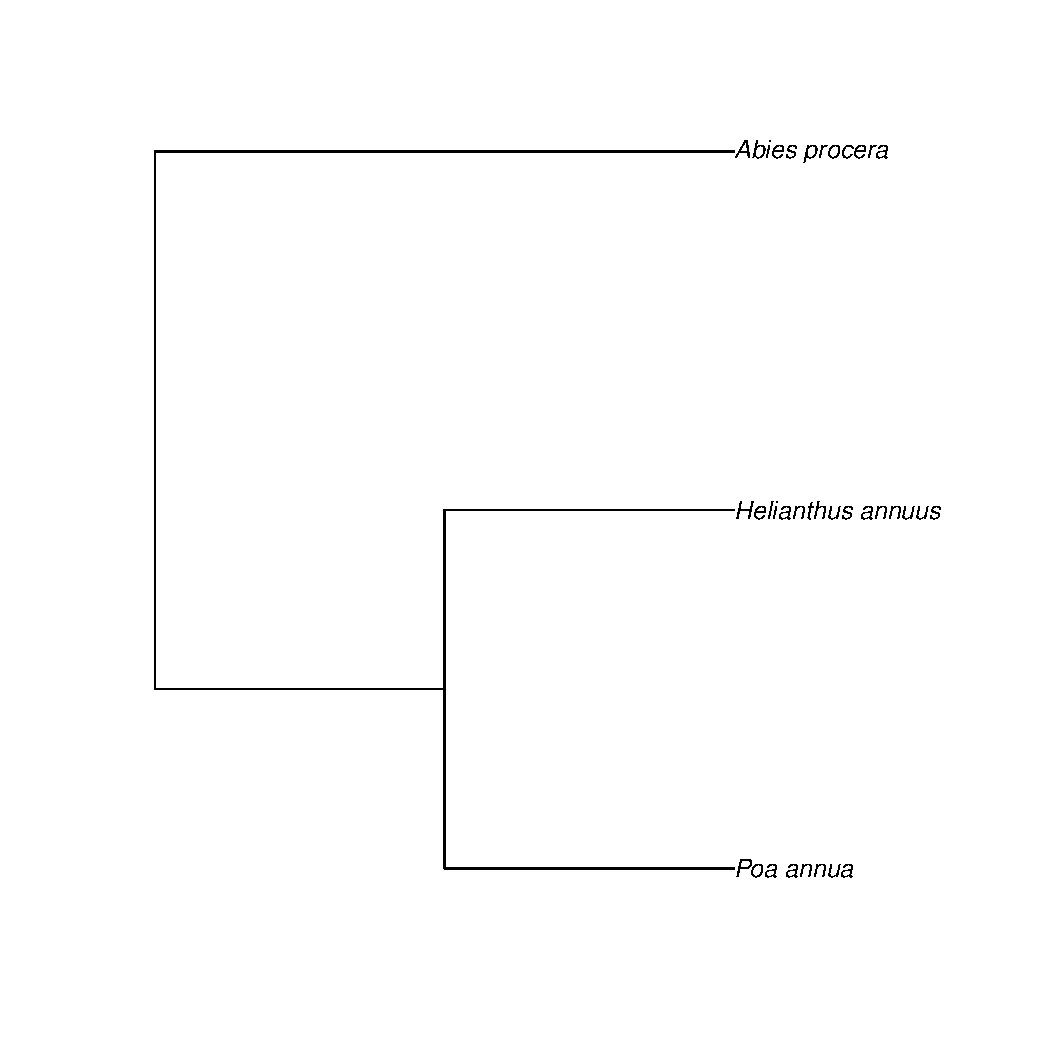
\includegraphics[width=.7\textwidth]{chapters/taxize/phylogeny.pdf}
\end{center}
\caption[A phylogeny for three species produced using the \emph{phylomatic\_tree} function.]{
{A phylogeny for three species. This phylogeny was produced using the \emph{phylomatic\_tree} function, which queries the Phylomatic database, and prunes a previously created phylogeny of plants.}
}
\label{fig:taxize:phylomatic}
\end{figure}

Behind the scenes the function \emph{phylomatic\_tree} retrieves a Taxonomic Serial Number (TSN) from ITIS for each species name, then a string is created for each species like this \emph{poaceae/oryza/oryzasativa} (with format "family/genus/\\genus\_epithet"). 
These strings are submitted to the Phylomatic API, and if no errors occur, a phylogeny in newick format is returned. 
The \emph{phylomatic\_tree()} function also cleans up the newick string and converts it to an ape \emph{phylo} object, which can be used for plotting and phylogenetic analyses. 
Be aware that Phylomatic has certain limitations - refer to the paper describing Phylomatic \citep{webb2005} and the website \url{http://phylodiversity.net/phylomatic/}.



\subsection{What taxa are children of the taxon of interest?}
If someone is not a taxonomic specialist on a particular taxon they probably do not know what children taxa are within a family, or within a genus. 
This task becomes especially unwieldy when there are a large number of taxa downstream. 
You can of course go to a website like Wikispecies (\url{http://species.wikimedia.org}) or Encyclopedia of Life (\url{http://eol.org/}) to get downstream names. 
However, taxize provides an easy way to programatically search for downstream taxa, both for the Catalogue of Life (CoL) (\url{http://www.catalogueoflife.org/}) and the Integrated Taxonomic Information System (\url{http://www.itis.gov/}). 
Here is a short example using the CoL in which we want to find all the species within the genus \emph{Apis} (honey bees).

\begin{knitrout}
\small
\definecolor{shadecolor}{rgb}{0.969, 0.969, 0.969}
\color{fgcolor}
\begin{kframe}
\begin{alltt}
\hlkwd{col_downstream}\hlstd{(}\hlkwc{name} \hlstd{=} \hlstr{"Apis"}\hlstd{,} \hlkwc{downto} \hlstd{=} \hlstr{"Species"}\hlstd{)[[}\hlnum{1}\hlstd{]]}
\end{alltt}
\begin{verbatim}
#   childtaxa_id     childtaxa_name childtaxa_rank
# 1      6971712 Apis andreniformis        Species
# 2      6971713        Apis cerana        Species
# 3      6971714       Apis dorsata        Species
# 4      6971715        Apis florea        Species
# 5      6971716 Apis koschevnikovi        Species
# 6      6845885     Apis mellifera        Species
# 7      6971717   Apis nigrocincta        Species
\end{verbatim}
\end{kframe}
\end{knitrout}

The result from the above call to \emph{col\_downstream()} is a data.frame that gives a number of columns of different information.


\subsection{IUCN Status}
There are a number of things a user can do once they have the correct taxonomic names. 
One thing a user can do is ask about the conservation status of a species (IUCN Red List of Threatened Species (\url{http://www.iucnredlist.org})). 
We have provided a set of functions, \emph{iucn\_summary} and \emph{iucn\_status}, to search for species names, and extract the status information, respectively. 
Here, you can search for the panther and lynx.

\begin{knitrout}\small
\definecolor{shadecolor}{rgb}{0.969, 0.969, 0.969}
\color{fgcolor}
\begin{kframe}
\begin{alltt}
\hlstd{ia} \hlkwb{<-} \hlkwd{iucn_summary}\hlstd{(}\hlkwd{c}\hlstd{(}\hlstr{"Panthera uncia"}\hlstd{,} \hlstr{"Lynx lynx"}\hlstd{))}
\hlkwd{iucn_status}\hlstd{(ia)}
\end{alltt}
\begin{verbatim}
# Panthera uncia      Lynx lynx 
#           "EN"           "LC"
\end{verbatim}
\end{kframe}
\end{knitrout}

It turns out that the panther has a status of endangered (EN) and the lynx has a status of least concern (LC).


\subsection{Search for available genes in GenBank}
Another use case available in taxize deals with genetic sequences. 
taxize has three functions to interact with GenBank to search for available genes \\ (\emph{get\_genes\_avail}), download genes by GenBank ID (\emph{get\_genes}), and download genes via taxonomic name search, including retrieving a congeneric if the searched taxon does not exist in the database (\emph{get\_seqs}). 
In this example, one can search for gene sequences for \emph{Umbra limi}.

\begin{knitrout}\small
\definecolor{shadecolor}{rgb}{0.969, 0.969, 0.969}\color{fgcolor}\begin{kframe}
\begin{alltt}
\hlstd{out} \hlkwb{<-} \hlkwd{get_genes_avail}\hlstd{(}\hlkwc{taxon_name} \hlstd{=} \hlstr{"Umbra limi"}\hlstd{,}
                       \hlkwc{seqrange} \hlstd{=} \hlstr{"1:2000"}\hlstd{,}
                       \hlkwc{getrelated} \hlstd{=} \hlnum{FALSE}\hlstd{)}
\end{alltt}
\end{kframe}
\end{knitrout}


Then one can ask if 'RAG1' exists in any of the gene names.

\begin{knitrout}\small
\definecolor{shadecolor}{rgb}{0.969, 0.969, 0.969}\color{fgcolor}\begin{kframe}
\begin{alltt}
\hlstd{out[}\hlkwd{grep}\hlstd{(}\hlstr{"RAG1"}\hlstd{, out}\hlopt{$}\hlstd{genesavail,} \hlkwc{ignore.case} \hlstd{=} \hlnum{TRUE}\hlstd{),} \hlopt{-}\hlnum{3}\hlstd{]}
\end{alltt}
\begin{verbatim}
#         spused length access_num       ids
# 413 Umbra limi    732   JX190826 394772608
# 427 Umbra limi    959   AY459526  45479841
# 434 Umbra limi   1631   AY380548  38858304
\end{verbatim}
\end{kframe}
\end{knitrout}


It turns out that there are 430 different unique records found. 
However, this doesn't mean that there are 430 different genes found as the API does not provide metadata to classify genes. 
You can use regular expressions (e.g., \emph{grep}) to search for the gene of interest.


\subsection{Matching species tables with different taxonomic resolution}
Biologists often need to match different sets of data tied to species. 
For example, trait-based approaches are a promising tool in ecology \citep{statzner_can_2010}. 
One problem is that abundance data must be matched with trait databases such as the NCBI Taxonomy database \citep{usseglio-polatera_biological_2000}. 
These two data tables may contain species information on different taxonomic levels and data might have to be aggregated to a joint taxonomic level, so that the data can be merged. 
taxize can help in this data-cleaning step, providing a reproducible workflow.

A user can use the mentioned \emph{classification}-function to retrieve the taxonomic hierarchy and then search the hierarchies up- and downwards for matches. 
Here is an example to match a species (A) with names of on different taxonomic levels (B1 \& B2).

\begin{knitrout}\small
\definecolor{shadecolor}{rgb}{0.969, 0.969, 0.969}\color{fgcolor}\begin{kframe}
\begin{alltt}
\hlstd{A} \hlkwb{<-} \hlstr{"gammarus roeseli"}
\hlstd{B1} \hlkwb{<-} \hlstr{"gammarus"}
\hlstd{B2} \hlkwb{<-} \hlstr{"gammaridae"}
\hlstd{A_clas} \hlkwb{<-} \hlkwd{classification}\hlstd{(A,} \hlkwc{db} \hlstd{=} \hlstr{'ncbi'}\hlstd{)}
\hlstd{B1_clas} \hlkwb{<-} \hlkwd{classification}\hlstd{(B1,} \hlkwc{db} \hlstd{=} \hlstr{'ncbi'}\hlstd{)}
\hlstd{B2_clas} \hlkwb{<-} \hlkwd{classification}\hlstd{(B2,} \hlkwc{db} \hlstd{=} \hlstr{'ncbi'}\hlstd{)}
\hlstd{A_clas[[}\hlnum{1}\hlstd{]]}\hlopt{$}\hlstd{Rank[}\hlkwd{tolower}\hlstd{(A_clas[[}\hlnum{1}\hlstd{]]}\hlopt{$}\hlstd{ScientificName)} \hlopt \hlstd{B1]}
\end{alltt}
\begin{verbatim}
# [1] "genus"
\end{verbatim}
\begin{alltt}
\hlstd{A_clas[[}\hlnum{1}\hlstd{]]}\hlopt{$}\hlstd{Rank[}\hlkwd{tolower}\hlstd{(A_clas[[}\hlnum{1}\hlstd{]]}\hlopt{$}\hlstd{ScientificName)} \hlopt \hlstd{B2]}
\end{alltt}
\begin{verbatim}
# [1] "family"
\end{verbatim}
\end{kframe}
\end{knitrout}

If one finds a direct match (here \emph{Gammarus roeseli}), they will be lucky. 
However, Gammaridae can also be matched with \emph{Gammarus roeseli}, but on a lower taxonomic level. 
A more comprehensive and realistic example (matching a trait table with an abundance table) is given in the supplemental materials.


\subsection{Aggregating data to a specific taxonomic rank}
In biology, one can ask questions at varying taxonomic levels. 
This use case is easily handled in taxize. 
A function called \emph{tax\_agg()} will aggregate community data to a specific taxonomic level. 
In this example, one can take the data for three species and aggregate them to family level. 
Again one can specify whether they want to use data from ITIS or NCBI. 
The rows in the \emph{data.frame} are different communities.

\begin{knitrout}\small
\definecolor{shadecolor}{rgb}{0.969, 0.969, 0.969}\color{fgcolor}\begin{kframe}
\begin{alltt}
\hlkwd{data}\hlstd{(dune,} \hlkwc{package} \hlstd{=} \hlstr{'vegan'}\hlstd{)}
\hlstd{df} \hlkwb{<-} \hlstd{dune[ ,} \hlkwd{c}\hlstd{(}\hlnum{1}\hlstd{,}\hlnum{3}\hlopt{:}\hlnum{4}\hlstd{)]}
\hlkwd{colnames}\hlstd{(df)} \hlkwb{<-} \hlkwd{c}\hlstd{(}\hlstr{"Bellis perennis"}\hlstd{,} \hlstr{"Juncus bufonius"}\hlstd{,}
                  \hlstr{"Juncus articulatus"}\hlstd{)}
\hlkwd{head}\hlstd{(df)}
\end{alltt}
\begin{verbatim}
#    Bellis perennis Juncus bufonius Juncus articulatus
# 2                3               0                  0
# 13               0               3                  0
# 4                2               0                  0
# 16               0               0                  3
# 6                0               0                  0
# 1                0               0                  0
\end{verbatim}
\end{kframe}
\end{knitrout}


\begin{knitrout}footnotesize
\definecolor{shadecolor}{rgb}{0.969, 0.969, 0.969}\color{fgcolor}\begin{kframe}
\begin{alltt}
\hlstd{agg} \hlkwb{<-} \hlkwd{tax_agg}\hlstd{(df,} \hlkwc{rank} \hlstd{=} \hlstr{'family'}\hlstd{,} \hlkwc{db} \hlstd{=} \hlstr{'ncbi'}\hlstd{)}
\hlstd{agg}
\end{alltt}
\begin{verbatim}
# 
# 	Aggregated community data
# 
# Level of Aggregation: FAMILY
# No. taxa before aggregation: 3
# No. taxa after aggregation: 2
# No. taxa not found: 0
\end{verbatim}
\end{kframe}
\end{knitrout}


\begin{knitrout}\small
\definecolor{shadecolor}{rgb}{0.969, 0.969, 0.969}\color{fgcolor}\begin{kframe}
\begin{alltt}
\hlkwd{head}\hlstd{(agg}\hlopt{$}\hlstd{x)}
\end{alltt}
\begin{verbatim}
#    Asteraceae Juncaceae
# 2           3         0
# 13          0         3
# 4           2         0
# 16          0         3
# 6           0         0
# 1           0         0
\end{verbatim}
\end{kframe}
\end{knitrout}

The two \emph{Juncus} species are aggregated to the family Juncaceae and their abundances are summed. 
There was only a single species in the family Asteraceae, so the data for \emph{Bellis perennis} are carried over.


%% ----------------------------------------------------------------------------
\section{Conclusions}
\label{sec:taxize:conclusions}
Taxonomic information is increasingly sought by biologists as we take phylogenetic and taxonomic approaches to science.
Taxonomic data are becoming more widely available on the web, yet scientists require programmatic access to this data for developing reproducible workflows.
taxize was created to bridge this gap - to bring taxonomic data on the web into R, where the data can be easily manipulated, visualized, and analyzed in a reproducible workflow.

We have outlined a suite of use cases in taxize that will likely fit real use cases for many biologists.
Of course we have not thought of all possible use cases, so we hope that the biology community can give us feedback on what use cases they want to see available in taxize.
One thing we could change in the future is to make functions that fit use cases, and then allow users to select the data source as a parameter in the function.
This could possibly make the user interface easier to understand.

taxize is currently under development and will be for some time given the large number of data sources knitted together in the package, and the fact that APIs for each data source can change, requiring changes in taxize code.
Contributions to taxize are strongly encouraged, and can be easily done using GitHub here: \url{https://github.com/ropensci/taxize}.
We hope taxize will be taken up by the community and developed collaboratively, making it progressively better through time as new use cases arise, bug reports are squashed, and contributions are merged.

%% ----------------------------------------------------------------------------
\section{References}
\printbibliography[heading=none]

\end{sloppypar}
